\iffalse
\documentclass[journal,12pt,twocolumn]{IEEEtran}
\usepackage{amsmath,amssymb,amsfonts,amsthm}
\usepackage{txfonts}
\usepackage{tkz-euclide}
\usepackage{listings}
\usepackage{gvv}
\usepackage[latin1]{inputenc}
\usepackage{adjustbox}
\usepackage{array}
\usepackage{tabularx}
\usepackage{pgf}
\usepackage{lmodern}
\usepackage{circuitikz}
\usepackage{tikz}
\usepackage{graphicx}
\usepackage[english]{babel}

\begin{document}
\bibliographystyle{IEEEtran}

\vspace{3cm}

\title{}
\author{EE23BTECH11047 - Deepakreddy P
}
\maketitle
\newpage
\bigskip

\noindent \textbf{32} \quad A single-phase full-bridge diode rectifier feeds a resistive load of $50 \Omega$ from a 200 V,
50 Hz single phase AC supply. If the diodes are ideal, then the active power, in watts,
drawn by the load is \rule{1cm}{0.5mm} (round off to nearest integer).  \\
\hfill (GATE EE 32)\\
\solution\\
\fi

\begin{figure}[ht]
  \centering
      \begin{circuitikz}[american]
   \draw (0,8) to [sV=200V](0,-1) to [short](6,-1) to [short](6,0) to [D,l=$D_3$](9,3);
   \draw (0,8) to [short](6,8) to [short](6,6);
   \draw (6,6) to [D,l=$D_1$](9,3);
   \draw (3,3) to [D,l=$D_4$](6,6);
   \draw (3,3) to [D,l=$D_2$](6,0);
   \draw (3,3) to [short](2.5,3) to [crossing, bipoles/crossing/size=1](2.5,-4.8) to [short](12,-4.8) to [R=50$\Omega$](12,3) to [short](9,3);
   \draw (9,3) to [short,i=\Large{I}](12,3);
\end{circuitikz}

  \caption{Circuit-1}
\end{figure}

\begin{figure}[ht]
   \centering
   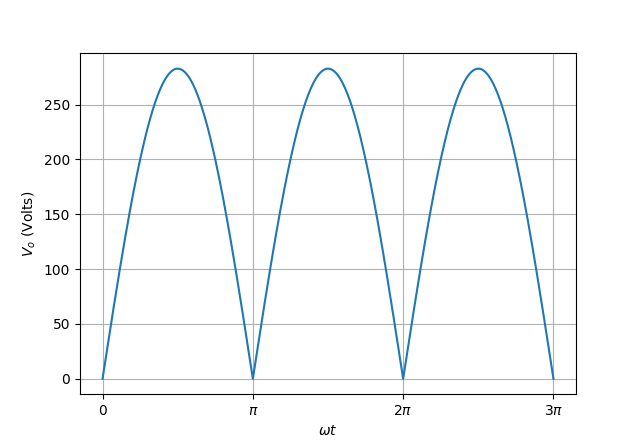
\includegraphics[width=1.2\columnwidth]{2022/EE/32/figs/gt1.png}
   \caption{Output voltage waveform of single-phase full
bridge rectifier}
\end{figure}


\begin{center}
    \begin{table}[ht]
        \setlength{\arrayrulewidth}{0.3mm}
\setlength{\tabcolsep}{12pt}
\renewcommand{\arraystretch}{1.3}


\begin{center}
\caption{Input Parameters}
\begin{tabular}{ |p{1.7cm}|p{1.7cm}|p{1.7cm}|  }

\hline
 {Symbol}&{Description} & {value}\\
\hline
R & Load Resistance & 50$\Omega$\\
\hline
$V_{rms}$ & RMS Voltage  & 200V\\
\hline
f & Frequency & 50Hz \\
\hline

\end{tabular}
\end{center}

    \end{table}
\end{center}

\begin{align}
    V_{rms} &= 200\\
    P &= \frac{\brak{V_{rms}}^2}{R}\\
    P &= \frac{\brak{200}^2}{50}W\\
    P &= 800W
\end{align}


%\end{document}

